\documentclass[a4paper,10pt]{article} % article

\usepackage[english]{babel}
\usepackage{graphicx}
\usepackage{subfig}
\usepackage{amsmath}
\usepackage{amssymb}
\usepackage{mathtools}
\usepackage{anysize}
\usepackage{pgfplots}
\usetikzlibrary{arrows.meta}
\tikzset{myarrow/.style={-{Triangle[length=3mm,width=1mm]}}}
\marginsize{2cm}{2cm}{2cm}{2cm}

%Highligh code
% Custom colors
\usepackage{color}
\definecolor{deepblue}{rgb}{0,0,0.5}
\definecolor{deepred}{rgb}{0.6,0,0}
\definecolor{deepgreen}{rgb}{0,0.5,0}
\definecolor{codegreen}{rgb}{0,0.5,0.2}
\definecolor{backcolour}{rgb}{0.95,0.95,0.92}

\usepackage{listings}

\lstdefinestyle{mystyle}{
    backgroundcolor=\color{backcolour},   
    commentstyle=\color{deepblue},
    keywordstyle=\color{codegreen},
    numberstyle=\tiny\color{deepgreen},
    stringstyle=\color{deepred},
    basicstyle=\footnotesize,
    breakatwhitespace=false,         
    breaklines=true,                 
    captionpos=b,                    
    keepspaces=true,                 
    numbers=left,                    
    numbersep=5pt,                  
    showspaces=false,                
    showstringspaces=false,
    showtabs=false,                  
    tabsize=2
}
 
\lstset{style=mystyle}

%Font
\usepackage{avant}
\usepackage[scaled]{helvet} % ss
\usepackage[helvet]{sfmath} 
\normalfont
\renewcommand*\familydefault{\sfdefault} %% Only if the base font of the document is to be sans serif
\usepackage[T1]{fontenc}
\usepackage{type1cm}
\usepackage{courier}
\renewcommand{\ttdefault}{pcr}
\DeclareMathAlphabet\mathbfcal{OMS}{cmsy}{b}{n}
 
 %Head and foot page
\usepackage{fancyhdr}
\pagestyle{fancy}
\fancyhf{}
\fancyhead[L]{ContactStructuralMechanicsApplication}
\fancyhead[R]{ALMFrictionlessMortarCondition}
\fancyfoot[R]{\leftmark}
\fancyfoot[L]{\thepage}
\renewcommand{\headrulewidth}{0.4pt}
\renewcommand{\footrulewidth}{0.4pt}
% \renewcommand{\headwidth}{17cm} 

\title{Augmented Lagrangian formulation for frictionless contact based in \em{Mortar} integration}
\author{Vicente Mataix Ferr\'andiz}
\date{June 2017}

\begin{document}

\maketitle

\section{Introduction}

The following document presents the formulation employed in the derivation of the frictionless \textit{Mortar} contact condition formulation with augmented dual \textit{Lagrange multiplier} (\textbf{ADLM}), based in the work of \textit{Alexander Popp}\cite{popp1,popp2} and \textit{Alberto Cardona}\cite{cardona1,cardona2}. The contact mechanics problems are based on the \textbf{IBVP} of non-linear solid mechanics and the unilateral contact constraints. After recapitulating some basic notation and the strong formulation, a weak formulation of the contact mechanics problems with two subdomains will be introduced.  In contrast to the mesh tying case considered so far, unilateral contact leads to a constrained minimization problem with inequality constraints, or more generally to so-called variational inequalities. It should be mentioned that both frictionless and frictional contact can either be formulated as variational inequalities with
a constrained solution or as saddle point problems based on \textit{Lagrange multipliers}, where the focus will be on the latter approach here. 

The motivation for dual \textit{Lagrange multipliers}\cite{wohlmuth} lies in the fact that an extension of the master side basis functions to the slave side of the interface has a global support for standard \textit{Lagrange multipliers}. 

\section{Content}

\subsection{Strong formulation}

On each subdomain $\Omega_0^{(i)}$ , the initial boundary value problem of finite deformation elastodynamics needs to be satisfied, viz \eqref{eq:eq0}.

\begin{subequations}\label{eq:eq0}
\begin{align}
 & \text{Div} \mathbf{P}^{(i)}+\hat{\mathbf{b}}_0^{(i)}=\rho_0^{(i)}\ddot{\mathbf{u}}^{(i)} \text{ in } \Omega_0^{(i)} \times [0, T] \label{eq:subeq1}\\
 & \mathbf{u}^{(i)} = \hat{\mathbf{u}}^{(i)} \text{ on } \Gamma_u^{(i)} \times [0, T] \label{eq:subeq2}\\
 & \mathbf{P}^{(i)} \cdot \mathbf{N}^{(i)} = \hat{\mathbf{t}}_0^{(i)} \text{ on } \Gamma_\sigma^{(i)} \times [0, T] \label{eq:subeq3} \\
 & \mathbf{u}^{(i)}\left( \mathbf{X}^{(i)}, 0\right) = \hat{\mathbf{u}}_0^{(i)}\left( \mathbf{X}^{(i)}\right) \text{ in } \Omega_0^{(i)} \label{eq:subeq4} \\
 & \dot{\mathbf{u}}^{(i)}\left( \mathbf{X}^{(i)}, 0\right) = \hat{\dot{\mathbf{u}}}_0^{(i)}\left( \mathbf{X}^{(i)}\right) \text{ in } \Omega_0^{(i)} \label{eq:subeq5}
 \end{align}
\end{subequations}

The contact constraints in normal direction are typically given in form of \textit{Karush-Kuhn-Tucker}\textbf{KKT} conditions as given in \eqref{eq:eq6}, and Figure \ref{fig:kkt}.
 
 \begin{equation}\label{eq:eq6}
g_n \geq 0 \text{ , } p_n \leq 0 \text{ , } p_n g_n = 0 \text{ on } \Gamma_c^{(i)} \times [0, T]
 \end{equation}

\begin{figure}[h]
\begin{center}
\begin{tikzpicture}
\begin{axis}[
%         grid= major ,
		width=0.8\textwidth ,
		xlabel style={font=\Large},
		xlabel = {$g_n$} ,
		ylabel style={font=\Large},
		ylabel = {$p_n$} ,
		xmin = -1, 
		xmax = 1,
		ymin = -1, 
		ymax = 1,
		axis lines=middle,
		axis line style={myarrow}
		]
\addplot[red, thick] expression[domain=-1:1, domain y=-1:1, samples=200] {(x>0? 0 : -10^9)}; 
\end{axis} 
\end{tikzpicture}
\caption{\textit{Karush–Kuhn–Tucker} (\textbf{KKT}) conditions of non-penetration.}
\label{fig:kkt}
\end{center}
\end{figure}

In the course of deriving a weak formulation, the balance of linear momentum at the unilateral contact problem  for the interface $\Gamma_c^{(i)}$ is typically exploited and a \textit{Lagrange multiplier} vector field $\lambda_n$ is introduced, thus setting the basis for a mixed variational approach. Unilateral contact constraints are typically
formulated (and later also numerically evaluated) in the current configuration.

\subsection{Weak formulation}

\subsubsection{Standard Lagrange multiplier}

To start the derivation of a weak formulation of \eqref{eq:eq0}, appropriate solution spaces $\mathbfcal{U}^{(i)}$ and
weighting spaces $\mathbfcal{V}^{(i)}$ need to be defined as \eqref{eq:eq7}.

\begin{equation}\label{eq:eq7}
 \begin{cases}
  \mathbfcal{U}^{(i)} = \left\{ \mathbf{u}^{(i)} \in H^1(\Omega) \| \mathbf{u}^{(i)} = \hat{\mathbf{u}}^{(i)} \text{ on } \Gamma_u^{(i)}\right\},\\
  \mathbfcal{V}^{(i)} = \left\{ \delta\mathbf{u}^{(i)} \in H^1(\Omega) \| \delta\mathbf{u}^{(i)} = \mathbf{0} \text{ on } \Gamma_u^{(i)}\right\}
 \end{cases}
\end{equation}

Additionally the \textit{Lagrange multiplier} vector $\boldsymbol{\lambda}_n = \lambda_n \cdot \mathbf{n} = -\mathbf{t}_c^{(1)}$, which enforce the unilateral contact constraint\eqref{eq:eq6}, represents the negative slave side contact traction $\mathbf{t}_c^{(1)}$, is chosen from a corresponding solution space denoted as $\mathbfcal{M}$.%chosen the convex cone $\mathbfcal{M}(\boldsymbol{\lambda}) \subset \mathbfcal{M}$ given by \eqref{eq:eq7_5}. \textonehalf TODO: This is for the frictional case

% \begin{equation}\label{eq:eq7_5}
%  \mathbfcal{M}(\boldsymbol{\lambda}) \left\{  \right\}
% \end{equation}

In terms of its classification in functional analysis, this space represents the dual space of the trace space $\mathbfcal{W}^{(1)}$ of $\mathbfcal{V}^{(1)}$. In the given context, this means that $\mathcal{M} = H^{−1/2} (\Gamma_c)$ and $\mathcal{W}^{(1)} = H^{1/2} (\Gamma_c)$, where $\mathcal{M}$  and $\mathcal{W}^{(1)}$ denote single scalar components of the corresponding vector-valued spaces $\mathbfcal{M}$ and $\mathbfcal{W}$.

Based on these considerations, a saddle point type weak formulation is derived next. This can be done by extending the standard weak formulation of non-linear solid mechanics as defined to two subdomains and combining it with the \textit{Lagrange multiplier} coupling terms introduced in generic form. Find $\mathbf{u}^{(i)} \in \mathbfcal{U}^{(i)}$ and $\lambda_n \in \mathbfcal{M}$ such that we obtain \eqref{eq:eqfunct0}, than once derived \eqref{eq:eqfunct}.

\begin{subequations}
\begin{equation}\label{eq:eqfunct0}
 \delta \mathcal{W}^{co}(\mathbf{u},\lambda_n) = \int_{\Gamma_c^{(1)}} \lambda_n \cdot g_n \text{d}A
\end{equation}

Where $g_n$ is the continuous normal gap, that can be defined as \eqref{eq:eqgap}.

\begin{equation}\label{eq:eqgap}
 g_n = \mathbf{n}^{(1)}\cdot\left( \mathbf{u}^{(1)} - \mathbf{u}^{(2)}\right)
\end{equation}
\end{subequations}

\begin{subequations}\label{eq:eqfunct}
 \begin{align}
\delta\mathcal{W}(\mathbf{u},\lambda_n) = \delta\mathcal{W}_\mathbfcal{V} + \delta\mathcal{W}_\mathbfcal{M} & \\
\delta\mathcal{W}_\mathbfcal{V} = -\delta \mathcal{W}_{kin}(\mathbf{u}^{(i)},\delta \mathbf{u}^{(i)}) - \delta \mathcal{W}_{int,ext}(\mathbf{u}^{(i)},\delta \mathbf{u}^{(i)}) & - \delta\mathcal{W}_{co}(\boldsymbol{\lambda}^{(i)},\delta \mathbf{u}^{(i)}) = 0 \text{ } \forall \delta \mathbf{u}^{(i)} \in  \mathbfcal{V} \label{eq:subeq8} \\ 
\delta\mathcal{W}_\mathbfcal{M} = & - \delta\mathcal{W}_{\lambda}(\mathbf{u}^{(i)},\delta \boldsymbol{\lambda}^{(i)}) \geq 0 \text{ } \forall \delta \boldsymbol{\lambda}^{(i)} \in  \mathbfcal{M} \label{eq:subeq9}
 \end{align}
\end{subequations}

Herein, the kinetic contribution $\delta \mathcal{W}_{kin}$ , the internal and external contributions $\delta \mathcal{W}_{int,ext}$ and the unilateral contact contribution $\delta\mathcal{W}_{co}$ to the overall virtual work on the two subdomains, as well as the weak form of the unilateral contact constraint $\delta\mathcal{W}_{\lambda}($, have been abbreviated as \eqref{eq:contributions}.

\begin{subequations}\label{eq:contributions}
 \begin{align}
  & -\delta \mathcal{W}_{kin} = \sum_{i = 1}^2 \left[\int_{\Omega_0^{(i)}} \rho_0^{(i)} \ddot{\mathbf{u}}^{(i)} \cdot \delta \mathbf{u}^{(i)} \text{d}V\right] \label{eq:subeq10} \\
 & -\delta \mathcal{W}_{int,ext} = \sum_{i = 1}^2 \left[\int_{\Omega_0^{(i)}} \left(\mathbf{S}^{(i)} : \delta \mathbf{E}^{(i)} - \hat{\mathbf{b}}\cdot \delta\mathbf{u}^{(i)} \right) \text{d}V - \int_{\Gamma_\sigma^{(i)}} \hat{\mathbf{t}}_0^{(i)}\cdot\delta\mathbf{u}^{(i)} \text{d}A \right] \label{eq:subeq11} \\
 & -\delta \mathcal{W}_{co} = \sum_{i = 1}^2 \left[\int_{\Gamma_c^{(i)}} \lambda_n \cdot \delta g_n \text{d}A\right] \label{eq:subeq12} \\ 
 & -\delta \mathcal{W}_{\lambda} = \sum_{i = 1}^2 \left[\int_{\Gamma_c^{(i)}} \delta \lambda_n \cdot g_n \text{d}A\right] \label{eq:subeq13}
 \end{align}
\end{subequations}

The coupling terms on $\Gamma_c$ also allow for a direct interpretation in terms of variational formulations and the principle of virtual work. Whereas the contribution in \eqref{eq:subeq12} represents the virtual work of the unknown interface tractions $\boldsymbol{\lambda} = −\mathbf{t}_c^{(1)} = \mathbf{t}_c^{(2)}$, the contribution in \eqref{eq:subeq13} ensures a weak, variationally consistent enforcement of the unilateral contact constraint \eqref{eq:eq6}. Nevertheless, the concrete choice of the discrete Lagrange multiplier space $\mathbfcal{M}_h$ in the context of mortar finite element discretisations is decisive for the stability of the method and for optimal a priori error bounds. Finally, it is pointed out that the weak formulation \eqref{eq:subeq8} and \eqref{eq:subeq9} possesses all characteristics of saddle point problems and \textit{Lagrange multiplier} methods.

In contrast to the mesh tying case, where this mapping only came into play in the discrete setting, $\gamma_c^{(1)}$ and $\gamma_c^{(2)}$ cannot even be guaranteed to be identical in the continuum framework for unilateral contact, because they not only comprise the actual contact surfaces but the potential contact surfaces. 

As compared with the mesh tying case, it is noticeable that the weak formulation contains inequality \eqref{eq:subeq9} conditions for unilateral contact. These require a particular numerical treatment based on active set strategies.

\subsubsection{Augmented Lagrange multiplier}

One of the main disadvantages of the standard \textit{Lagrange multiplier} is the saddle point problem that appears in the formulation. For solving that, an \textbf{Augmented Lagrangian} method to solve contact problems with friction was proposed by \textit{Alart and Curnier}\cite{alart} based on a reformulation of the contact and friction laws into a system
of equations without inequalities. 

Focusing in the functional relative to the contact ($\mathcal{W}^{co}(\mathbf{u},\lambda_n) = \mathcal{W}^{co}_\mathbfcal{V} + \mathcal{W}_\mathbfcal{M}$), we can rewrite \eqref{eq:eqfunct0} as \eqref{eq:eqalmfunct0}.

\begin{equation}\label{eq:eqalmfunct0}
 \mathcal{W}^{co}(\mathbf{u},\lambda_n) = \int_{\Gamma_c^{(1)}} k \lambda_n \cdot g_n  + \frac{\varepsilon}{2} g_n^2 - \frac{1}{2\varepsilon} \langle k \lambda_n + \varepsilon g_n \rangle^2\text{d}A
\end{equation}

Where $\varepsilon$ is a positive penalty parameter, $k$ is a positive scale factor, and $\langle \rangle$ is the \textit{Macauley} bracket operator, that is \eqref{eq:eqmac}.

\begin{equation}\label{eq:eqmac}
 \langle x \rangle \begin{cases} x \text{ } x \geq 0\\ 0 \text{ } x < 0 \end{cases}
\end{equation}

This functional is $\mathcal{C}^1$ differentiable saddle-point, as shown in Figure \ref{fig:locusalm}. The solution is obtained as the set of values that render this functional stationary. 

\begin{figure}[h]
\begin{center}
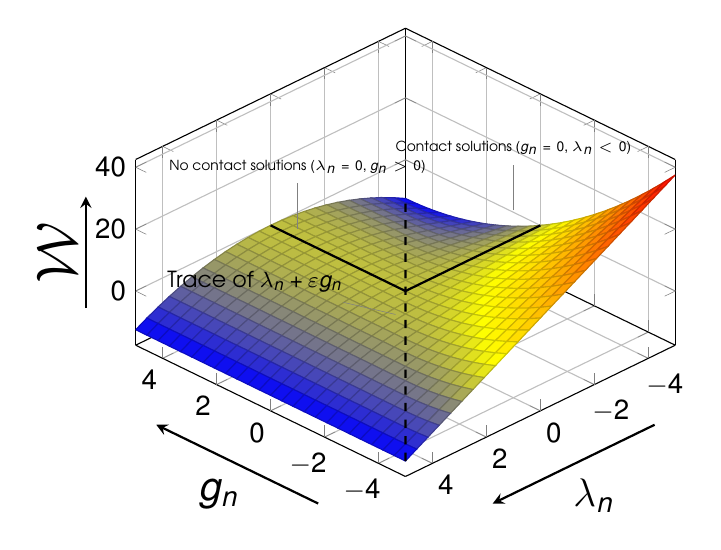
\begin{tikzpicture}[
declare function={functional(\r,\k)={(\k*y+\r*x > 0 ? \k*y*x+\r*0.5*x^2-0.5/\r*(\k*y+\r*x)^2:\k*y*x+\r*0.5*x^2)};}
]
\begin{axis}[grid=both, 
%             title= Augmented Lagrangian function for the contact problem,
            xlabel={$g_n$},
            xticklabel pos=left, 
            xlabel style={font=\Large},
            ylabel={$\lambda_n$},
            x dir=reverse,
            yticklabel pos=left, 
            ylabel style={font=\Large},
            y dir=reverse,
            zlabel={$\mathcal{W}$},
            zticklabel pos=left, 
            zlabel style={font=\huge},
            after end axis/.code={
                \draw [-stealth, thick, black] (xticklabel cs:0.8) -- (xticklabel cs:0.2);
                \draw [-stealth, thick, black] (yticklabel cs:0.8) -- (yticklabel cs:0.2);
                \draw [-stealth, thick, black] (zticklabel cs:0.2) -- (zticklabel cs:0.8);                
            }
            ,unbounded coords = jump
            ,view = {45}{45}
%             ,colormap name  = whitered
%             ,colorbar style = {
%                 at     = {(1,0)},
%                 anchor = south west,
%                 height = 0.25*\pgfkeysvalueof{/pgfplots/parent axis height},
%                 title  = {$\mathcal{W}$}
%                 }
            ]
\addplot3[surf,shader=faceted]{functional(1.0,1.0)};
\addplot3[samples=30,samples y=0, thick, dashed ,black,smooth]({x},{-x},{-0.5*x^2});
\addplot3[samples=30, domain=5:0, samples y=0, thick,black,smooth]({x},{0.0},{0.0});
\addplot3[samples=30, domain=0:-5,samples y=0, thick,black,smooth]({0.0},{x},{0.0});
\node at (axis cs: 4.0,0.0,0.0 ) [pin=90:\tiny{No contact solutions  $(\lambda_n=0,g_n>0)$}] {};
\node at (axis cs: 0.0,-4.0,6.0) [pin=90:\tiny{Contact solutions $(g_n=0,\lambda_n<0)$}] {};
\node at (axis cs:-1,1,0.18) [pin=165:\footnotesize{Trace of $\lambda_n+\varepsilon g_n$}] {};
\end{axis}
\end{tikzpicture}
\caption{Augmented Lagrangian function for the contact problem. The locus of solutions is displayed.}
\label{fig:locusalm}
\end{center}
\end{figure}

The solution does not depend on the value of parameters $\varepsilon$ and $k$. Nevertheless, the convergence rate does depend on their value. In numerical computations, default values of $\varepsilon$ and $k$ are selected in terms of a mean value of the \textit{Young} modulus of the bodies in contact and of a mean value of mesh size, as \eqref{eq:eqcoeff}. Numerical examples show that this choice gives a better condition number of the iteration matrix than other choices. 

\begin{equation}\label{eq:eqcoeff}
 \varepsilon = k \approx 10 \frac{E_{mean}}{h_{mean}}
\end{equation}

The functional \eqref{eq:eqalmfunct0} can be separated in two different parts, as can be seen in \eqref{eq:eqalmfunct1}.

\begin{equation}\label{eq:eqalmfunct1}
  \mathcal{W}^{co}(\mathbf{u},\lambda_n) = \int_{\Gamma_c^{(1)}} \begin{cases}  k \lambda_n \cdot g_n  + \frac{\varepsilon}{2} g_n^2 \text{d}A & \text{ if } k\lambda_n +\varepsilon g_n \leq 0 \text{ (Contact zone)} \\ - \frac{k}{2\varepsilon} \lambda_n^2   & \text{ if } k\lambda_n +\varepsilon g_n > 0 \text{ (Gap zone)} \end{cases}\text{d}A 
\end{equation}

Finally we can derive \eqref{eq:eqalmfunct1} to obtain the variational form from \eqref{eq:eqalmfunct2}, where to simplify we define the augmented normal pressure $\hat{\boldsymbol{\lambda}}_{n} = k\lambda_n +\varepsilon g_n $.

\begin{equation}\label{eq:eqalmfunct2}
  \delta \mathcal{W}^{co}(\mathbf{u},\lambda_n) = \int_{\Gamma_c^{(1)}}\begin{cases}  \hat{\boldsymbol{\lambda}}_{n} \cdot \delta g_n + k g_n \delta\lambda_n & \text{ if } \hat{\boldsymbol{\lambda}}_{n} \leq 0 \text{ (Contact zone)} \\  - \frac{k^2}{\varepsilon} \lambda_n \delta\lambda_n & \text{ if } \hat{\boldsymbol{\lambda}}_{n} > 0 \text{ (Gap zone)} \end{cases} \text{d}A 
\end{equation}

The functional from \eqref{eq:eqalmfunct2} makes that the system obtained varies in function if the nodes are present in the contact or the gap zone, so the system is not a priori known and in the following to present the numerical discretisation will focus in the solution obtained in the gap zone. Once this is derived the solution in the gap zone can be obtained in a in a straight-forward way.

\subsection{Discretisation and numerical integration}

\subsubsection{Dual Lagrange multipliers}

\paragraph{Definition}:

The discretisations of the displacements correspond with the standard ones in the finite element formulation, for more information check the literature\cite{Zienkiewicz1}. In addition, an adequate discretisation of the Lagrange multiplier vector $\boldsymbol{\lambda}$ is needed, and will be based on a discrete \textit{Lagrange multiplier} space $\mathbfcal{M}_h$ being an approximation of $\mathbfcal{M}$. Thus, we can define the discete \textit{Lagrange multiplier} as \eqref{eq:eq14}, with the shape functions $\Phi_j$ and the discrete nodal Lagrange multipliers $\boldsymbol{\lambda}_h$.

\begin{equation}\label{eq:eq14}
 \boldsymbol{\lambda}_h = \sum_{i=1}^{m^{(1)}} \Phi_j\left(\xi^{(1)},\eta^{(1)} \right) \boldsymbol{\lambda}_j
\end{equation}

Details on how to define dual Lagrange multiplier shape functions $\Phi_j$ using the so-called biorthogonality relationship with the standard displacement shape functions $N_k$ have first been presented in \textit{Wohlmuth}\cite{wohlmuth}. A common notation of the biorthogonality condition is \eqref{eq:eq15}.

\begin{equation}\label{eq:eq15}
 \int_{\Gamma_{c,h}^{(1)}}\Phi_j N_k^{(1)} \text{d}A = \delta_{jk} \int_{\Gamma_{c,h}^{(1)}} N_k^{(1)} \text{d}A \text{ , } j,k=1,...,m^{(1)}
\end{equation}

Herein, $\delta_{jk}$ is the \textit{Kronecker} delta, and the most common choice $m^{(1)} = n^{(1)}$ is assumed. For
practical reasons, the biorthogonality condition is typically applied locally on each slave element $e$, yielding \eqref{eq:eq16}, where $m_e^{(1)}$ represents the number of Lagrange multiplier nodes of the considered slave element.

\begin{equation}\label{eq:eq16}
 \int_{e}\Phi_j N_k^{(1)} \text{d}e = \delta_{jk} \int_{e} N_k^{(1)} \text{d}e \text{ , } j,k=1,...,m_e^{(1)}
\end{equation}

Combining the biorthogonality condition in \eqref{eq:eq16} and the partition of unity property of the dual shape functions, it follows that \eqref{eq:eq17}.

\begin{equation}\label{eq:eq17}
 \int_e \Phi_j de =  \int_e N_j^{(1)} de \text{ , } j=1,...,m_e^{(1)}
\end{equation}

It is important to point out that the elementwise biorthogonality condition in \eqref{eq:eq16} must be satisfied in the physical space, and not simply in the finite element parameter space. Consequently, a matrix system of size $m_e^{(1)} \times m_e^{(1)}$ must be solved on each slave element. The first step for doing this is to introduce unknown linear coefficients $a_{jk}$ such that \eqref{eq:eq18}.

\begin{equation}\label{eq:eq18}
 \Phi_j(\xi, \eta) = a_{jk} N_k^{(1)}\left(\xi, \eta \right), \mathbf{A}_e = [a_{jk}] \in \mathbb{R}^{m_e^{(1)} \times m_e^{(1)}}
 \end{equation}
 
 It can easily be verified that, as second step, insertion of \eqref{eq:eq18} into \eqref{eq:eq16} yields the unknown
coefficient matrix $\mathbf{A}_e$ as \eqref{eq:eq19}, where $J(\xi, \eta)$ is the slave \textit{Jacobian} determinant.

\begin{equation}\label{eq:eq19}
\begin{aligned}
 & \mathbf{A}_e = \mathbf{D}_e\mathbf{M}_e^{-1} \\
 & \mathbf{D}_e = [d_{jk}] \in \mathbb{R}^{m_e^{(1)} \times m_e^{(1)}}, d_{jk} = \delta_{jk} \int_e N_k^{(1)}(\xi, \eta) J(\xi, \eta) \text{d}e \\
 & \mathbf{M}_e = [m_{jk}] \in \mathbb{R}^{m_e^{(1)} \times m_e^{(1)}}, m_{jk} = \int_e N_j^{(1)}(\xi, \eta) N_k^{(1)}(\xi, \eta) J(\xi, \eta) \text{d}e
\end{aligned}
 \end{equation}

\paragraph{Derivatives}:

To define $\Delta \phi$ it is necessary to define the derivatives from \eqref{eq:eq19}, which can be obtained with \eqref{eq:eq19b}.

\begin{equation}\label{eq:eq19b}
\begin{aligned}
 & \Delta \mathbf{A}_e = \Delta \mathbf{D}_e\mathbf{M}_e^{-1} - \mathbf{D}_e\Delta\mathbf{M}_e\mathbf{M}_e^{-1} \\
 &\Delta \mathbf{D}_e = \Delta[d_{jk}] \in \mathbb{R}^{m_e^{(1)} \times m_e^{(1)}}, \Delta d_{jk} = \delta_{jk} \sum_{g = 1}^{n_{gp}} w_g N_{gk}^{(1)} \Delta J_g^{(1)}  \\
 & \Delta \mathbf{M}_e = \Delta[m_{jk}] \in \mathbb{R}^{m_e^{(1)} \times m_e^{(1)}}, \Delta m_{jk} = \sum_{g = 1}^{n_{gp}} w_g  \sum_{g = 1}^{n_{gp}} w_g  N_{gj}^{(1)} N_{gk}^{(1)} \Delta J_g^{(1)}
\end{aligned}
 \end{equation}
 
\subsubsection{Mortar operators}

\paragraph{Definition}:

Considering the discrete \textit{Lagrange multiplier}\eqref{eq:eq14} in \eqref{eq:subeq8} we obtain \eqref{eq:eq20}, where $\chi_h$ is the interface mapping.

\begin{equation}\label{eq:eq20}
 -\delta \mathcal{W}_{co,h} = \sum_{j=1}^{m^{(1)}}\sum_{k=1}^{n^{(1)}} \boldsymbol{\lambda}_{nj}^T \left(\int_{\Gamma_{c,h}^{(1)}} \Phi_j N_k^{(1)} \text{d}A \right) \delta \mathbf{d}_{nk}^{(1)} -\sum_{j=1}^{m^{(1)}}\sum_{l=1}^{n^{(2)}} \boldsymbol{\lambda}_{nj}^T \left(\int_{\Gamma_{c,h}^{(1)}} \Phi_j \left(N_l^{(2)} \circ \chi_h\right) \text{d}A \right) \delta \mathbf{d}_{nl}^{(2)}
\end{equation}

Numerical integration of the mortar coupling terms is exclusively performed on the slave side $\Gamma_{c,h}$ of the interface. In \eqref{eq:eq20}, nodal blocks of the two mortar integral matrices commonly denoted as $\mathbf{D}$ and $\mathbf{M}$ can be identified. This leads to the following definitions \eqref{eq:eq21}.

 \begin{subequations}\label{eq:eq21}
 \begin{align}
 & \mathbf{D}[j,k] = D_{jk} \mathbf{I}_{ndim} = \int_{\Gamma_{c,h}^{(1)}} \Phi_j N_k^{(1)}\text{d}A\mathbf{I}_{ndim}\text{ , } j=1,...m^{(1)}\text{ , } k= 1, ...n^{(1)} = \sum_{g = 1}^{n_{gp}} w_g \phi_{gj} N_{gk}^{(1)} J_g^{(1)} \\
 & \mathbf{M}[j,l] = M_{jl} \mathbf{I}_{ndim} = \int_{\Gamma_{c,h}^{(1)}} \Phi_j \left(N_l^{(2)} \circ \chi_h \right)\text{d}A\mathbf{I}_{ndim}\text{ , } j=1,...m^{(1)}\text{ , } k= 1, ...n^{(2)} = \sum_{g = 1}^{n_{gp}} w_g \phi_{gj} N_{gk}^{(2)} J_g^{(1)} 
 \end{align}
\end{subequations}

Wit these matrices we can express the functional \eqref{eq:eq20} in the following way \eqref{eq:eq22}.

\begin{equation}\label{eq:eq22}
 -\delta \mathcal{W}_{co,h} = \delta \mathbf{x}_{n\mathcal{S}}^T\mathbf{D}^T\lambda_n - \delta \mathbf{x}_{n\mathcal{M}}^T\mathbf{M}^T\lambda_n = \delta \mathbf{x}_n \underbrace{\left[\begin{array}{c} \mathbf{0} \\ -\mathbf{M}^T \\ \mathbf{D}^T\end{array} \right]}_{\mathbf{B}^T_{co}} \lambda_n = \delta \mathbf{x}_n^T \mathbf{f}_{co}(\lambda_n)
\end{equation}

Herein, the discrete mortar unilateral contact operator $\mathbf{B}_{co}$ and the resulting discrete vector of unilateral contact forces $\mathbf{f}_{co} (\lambda_n) = \mathbf{B}_{co}\lambda_n$ acting on the slave and the master side of the interface are introduced. 

To finalize the discretisation of the considered unilateral contact problem, a closer look needs to
be taken at the weak constraint contribution $\delta \mathcal{W}_{\lambda,h} $ in \eqref{eq:subeq9}. Due to the saddle point characteristics and resulting symmetry of the mixed variational formulation in \eqref{eq:subeq8}  and \eqref{eq:subeq9}, all discrete components of $\delta \mathcal{W}_{\lambda,h}$ have already been introduced and the final formulation is given as \eqref{eq:eq23}, with $\mathbf{g}_{n}(\mathbf{x}) = \mathbf{B}_{mt} \mathbf{x} \cdot \mathbf{n}$ representing the discrete unilateral contact constraint at the coupling interface.

\begin{equation}\label{eq:eq23}
 -\delta \mathcal{W}_{\lambda,h} = \delta \lambda_n^T\mathbf{D}\mathbf{x}_{n\mathcal{S}} - \delta \lambda_n^T\mathbf{M}\mathbf{x}_{n\mathcal{M}}= \delta \lambda_n^T \mathbf{B}_{mt} \mathbf{x} \cdot \mathbf{n} = \delta \lambda_n^T \mathbf{g}_{n}(\mathbf{x})
\end{equation}

This discrete form of $\mathbf{g}_{n}$ can be renamed as nodal weighted gap for each node ($\tilde{g}_n$). 

\paragraph{Derivatives}:

To obtain a fully quadratic convergence in the computation of the contact problem we should compute the derivatives of the \textit{Mortar} operators, in consequence the derivatives of the \textit{Mortar} operators can be defined as \eqref{eq:eq24}.

\begin{subequations}\label{eq:eq24}
\begin{equation}
 \begin{aligned}
 \Delta\mathbf{D}[j,k] & = \Delta D_{jk} \mathbf{I}_{ndim} = \Delta  \int_{\Gamma_{c,h}^{(1)}} \Phi_j N_k^{(1)}\text{d}A\mathbf{I}_{ndim}\text{ , } j=1,...m^{(1)}\text{ , } k= 1, ...n^{(1)} \\ 
 & = \sum_{g = 1}^{n_{gp}} w_g \Delta\phi_{gj}        N_{gk}^{(1)}        J_g^{(1)} + \sum_{g = 1}^{n_{gp}} w_g       \phi_{gj} \Delta N_{gk}^{(1)}        J_g^{(1)} + \sum_{g = 1}^{n_{gp}} w_g        \phi_{gj}       N_{gk}^{(1)} \Delta J_g^{(1)} 
 \end{aligned}
 \end{equation}
 \begin{equation}
 \begin{aligned}
 \Delta\mathbf{M}[j,l]  & = \Delta M_{jl} \mathbf{I}_{ndim}  = \Delta  \int_{\Gamma_{c,h}^{(1)}} \Phi_j \left(N_l^{(2)} \circ \chi_h \right)\text{d}A\mathbf{I}_{ndim}\text{ , } j=1,...m^{(1)}\text{ , } k= 1, ...n^{(2)} \\
 & = \sum_{g = 1}^{n_{gp}} w_g \Delta\phi_{gj}        N_{gk}^{(2)}        J_g^{(1)}  + \sum_{g = 1}^{n_{gp}} w_g       \phi_{gj} \Delta N_{gk}^{(2)}        J_g^{(1)}  + \sum_{g = 1}^{n_{gp}} w_g        \phi_{gj}       N_{gk}^{(2)} \Delta J_g^{(1)} 
 \end{aligned}
 \end{equation}
\end{subequations}

\subsubsection{Matrix form of the problem}

%% TODO: Complete with all the casuistry 

Finally, once computed the mortar operators, the resulting system for unilateral contact corresponds (for fully activated system) with \eqref{eq:eq24}.

\begin{equation}\label{eq:eq24}
 \left[ \begin{array}{cccc} \mathbf{K}_{\mathcal{N}\mathcal{N}} &  \mathbf{K}_{\mathcal{N}\mathcal{M}} & \mathbf{K}_{\mathcal{N}\mathcal{S}} & \mathbf{0} \\ \mathbf{K}_{\mathcal{N}\mathcal{N}}  & \mathbf{K}_{\mathcal{M}\mathcal{M}} & \mathbf{0} & -(\mathbf{M}\cdot \mathbf{n})^{T} \\ \mathbf{K}_{\mathcal{S}\mathcal{N}} & \mathbf{0} & \mathbf{K}_{\mathcal{S}\mathcal{S}} & (\mathbf{D}\cdot \mathbf{n})^T \\ \mathbf{0} & -(\mathbf{M}\cdot \mathbf{n}) & (\mathbf{D}\cdot \mathbf{n}) & \mathbf{0}   \end{array} \right] \left[ \begin{array}{c} \Delta\mathbf{d}_{\mathcal{N}} \\ \Delta\mathbf{d}_{\mathcal{M}} \\ \Delta\mathbf{d}_{\mathcal{S}} \\ \Delta\lambda_n \end{array} \right] = - \left[ \begin{array}{c} \mathbf{r}_{\mathcal{N}} \\ \mathbf{r}_{\mathcal{M}} \\ \mathbf{r}_{\mathcal{S}} \\ g_n \end{array} \right] 
\end{equation}

\subsection{Active set strategy (Semismoth Newton Raphson)}

As mentioned before, the fully discrete problem statement of unilateral contact causes one major additional complexity with regard to global solution schemes as compared with the mesh tying case, namely the contact specific inequality constraints, which divide the set of all discrete constraints into two a priori unknown sets of active and inactive constraints. Mathematically speaking, this introduces an additional source of non-linearity apart from the well-known geometrical and material non-linearities of non-linear solid mechanics. To resolve this contact non-linearity, so-called primal-dual active set strategies (\textbf{PDASS}) will be employed.

The idea of any active set strategy in the context of unilateral contact is to find the correct subset of all slave nodes which are in contact with the master surface at the end of the currently considered time interval. The \textbf{PDASS} in  suffers from a serious drawback: the contact non-linearity, finding the correct active set A can not be resolved by a \textit{Newton–Raphson} type approach. 

The basic idea of an alternative \textbf{PDASS} formulation is to re-arrange the \textbf{KKT} conditions such that a \textit{Newton–Raphson} type algorithm can be applied not only for geometrical and material non-linearities, but also for the non-linearity stemming from contact itself, i.e. the active set search. So we reformulate the discrete \textbf{KKT} conditions within a so-called non-linear complementarity (\textbf{NCP}) function (Figure \ref{fig:ncp}). This function in the case of frictionless case basically corresponds with the augmented normal contact pressure $\hat{\boldsymbol{\lambda}}_n$ presented before, and the criteria will be to activate/inactivate the corresponding node when the augmented contact pressure is in compression or traction correspondingly. 

\begin{figure}[h]
\begin{center}
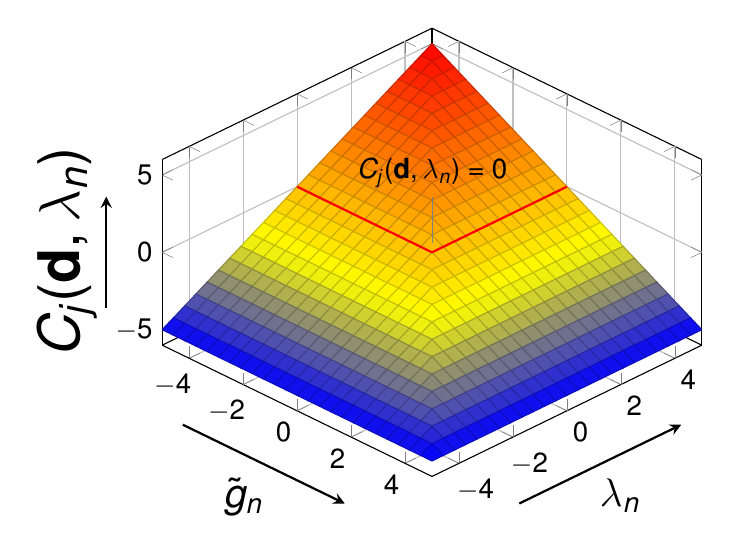
\begin{tikzpicture}[
declare function={myfunction(\r,\k)={\k*y - max(0, \k*y+\r*x)};}
]
\begin{axis}[grid=both, 
            xlabel={$\tilde{g}_n$},
            xticklabel pos=left, 
            xlabel style={font=\Large},
            ylabel={$\lambda_n$},
            yticklabel pos=left, 
            ylabel style={font=\Large},
            zlabel={$C_j(\mathbf{d}, \lambda_n)$},
            zticklabel pos=left, 
            zlabel style={font=\huge},
            after end axis/.code={
                \draw [-stealth, thick, black] (xticklabel cs:0.2) -- (xticklabel cs:0.8);
                \draw [-stealth, thick, black] (yticklabel cs:0.2) -- (yticklabel cs:0.8);
                \draw [-stealth, thick, black] (zticklabel cs:0.2) -- (zticklabel cs:0.8);                
            }
            ,unbounded coords = jump
            ,view = {45}{45}
            ]
\addplot3[surf,shader=faceted]{myfunction(1.0,1.0)};
\addplot3[samples=30, domain=-5:0, samples y=0, thick,red,smooth]({x},{0.0},{0.0});
\addplot3[samples=30, domain= 0:5,samples y=0, thick,red,smooth]({0.0},{x},{0.0});
\node at (axis cs: 0.0,0.0,0.0 ) [pin=90:\normalsize{$C_j(\mathbf{d}, \lambda_n) = 0$}] {};
\end{axis}
\end{tikzpicture}
\caption{Exemplary nodal \textbf{NCP} function $\hat{\boldsymbol{\lambda}}_n$ the normal part of the nodal weighted
gap $\tilde{g}_n$ and the nodal normal contact pressure $\lambda_n$. The equivalence with the \textbf{KKT} conditions is indicated in red colour.
}
\label{fig:ncp}
\end{center}
\end{figure}

Thus, the resulting \textbf{PDASS} contains derivative information on the sets themselves and allows for the application of a \textit{Newton–Raphson} type solution scheme also for the non-linearity stemming from contact. Consequently, all sources of non-linearities, i.e. finite deformations, non-linear material behaviour and contact itself, can be treated
within one single iterative scheme.

\begin{thebibliography}{99}

\bibitem{popp1} Popp, Alexander {\em Mortar Methods for Computational Contact Mechanics and General Interface Problems}  2012.

\bibitem{popp2}  Popp, Alexander and Gitterle, Markus and Gee, Michael W. and Wall, Wolfgang A. {\em A dual mortar approach for 3D finite deformation contact with consistent linearization} 2010: International Journal for Numerical Methods in Engineering

\bibitem{alart}   Alart P, Curnier A.  {\em A mixed formulation for frictional contact problems prone to Newton like solution methods.} 1991: Computer Methods in Applied Mechanics and Engineering; 92:353–375.

\bibitem{cardona1}  Calavalieri, FJ and Cardona, Alberto {\em An augumented lagrangian method to solve three-dimensional nonlinear contact problems} 2012: Latin American applied research

\bibitem{cardona2}  Calavalieri, FJ and Cardona, Alberto {\em An augmented Lagrangian technique combined with a mortar algorithm for modelling mechanical contact problems} 2013: International Journal for Numerical Methods in Engineering

\bibitem{wohlmuth} B. I. Wohlmuth,{\em Discretization methods and iterative solvers based on domain decomposition}, Springer-Verlag Berlin Heidelberg, 2001.

\bibitem{Zienkiewicz1} Zienkiewicz, O. C. and Zhu, J.Z. and Taylor, Robert L.,{\em The Finite Element Method: its Basis and Fundamentals}, Butterworth-Heinemann, 2013.

\end{thebibliography}

\end{document}
